\chapter{Conclusion and Future Work}
\label{chap:conclusion}
\begin{figure}[H] 
	\centering 
	\label{fig:demo}
	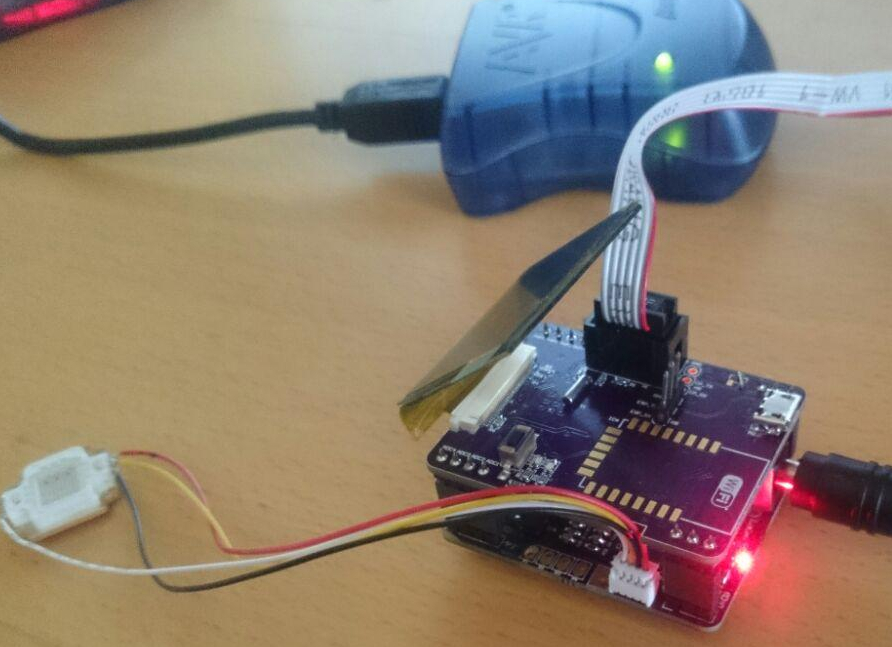
\includegraphics[width=0.6\textwidth]{./fig/demo.jpg}
	\caption{Picture of integrated system with ISP programmer.} 
\end{figure} Swakeup has still the
status of a prototype and room for improvement. There are
still a lot of things, which have to be done. The basic functionality is given
though. The most difficult part about this work is the simultaneous
development of hardware and software by the same person. On the one hand one
learns a lot and understands the interplay between both worlds better every day. On
the other hand it is quite challenging and one begins to realize, why
in industry software and hardware is developed seperately.  \newpar This wakeup
light differs in the sense of some significant improvements from the
state-of-the-art such as USB charging, email notification and and elegant,
highly-integrated design. Swakeup, once it is finished, is something quite
usefull, every Swede should have standing on his or her bedside table, not only because it can contribute to a healthier lifestyle in winter and hence to a happier society. 
